\documentclass[a4paper]{article}
\usepackage[italian]{babel}
\usepackage[italian]{isodate}  		% formato delle date in italiano
\usepackage{graphicx}				% gestione delle immagini
\usepackage{amsfonts}
\usepackage{booktabs}				% tabelle di qualità superiore
\usepackage{amsmath}				% pacchetto matematica
\usepackage{enumitem}				% gestione delle liste
\usepackage{pifont}					% pacchetto con elenchi carini
\usepackage[x11names]{xcolor}		% colori aggiuntivi
% Link ipertestuali per l'indice
\usepackage{xcolor}
\usepackage[linkcolor=black, citecolor=blue, urlcolor=cyan]{hyperref}
\hypersetup{
	colorlinks=true
}

%\usepackage{showframe}				% visualizzazione bordi
%\usepackage{showkeys}				% visualizzazione etichetta

\begin{document}
	\author{VR443470}
	\title{Analisi II}
	\date{\printdayoff\today}
	\maketitle
	
	\newpage
	
	% indice
	\tableofcontents
	
	\newpage
	
	%%%%%%%%%%%%%%
	% LEZIONE 01 %
	%%%%%%%%%%%%%%
	\section{Lezione 01}
	
	\subsection{Equazioni a variabili separabili}
	
	Le equazioni differenziali a \textbf{variabili separabili} hanno due forme:
	
	\begin{itemize}
		\item \textbf{Forma canonica.} $y'(x) = f(x)\cdot g\left(y(x)\right)$
		\item \textbf{Forma alternativa.} $y' = f(x) \cdot g(y)$
	\end{itemize}
	
	\noindent
	Dove $f$ e $g$ sono funzioni continue ``in un intervallo reale'', più formalmente:
	
	\begin{gather*}
		f \text{ continua in } I \subseteq R \\
		g \text{ continua in } J \subseteq R
	\end{gather*}
	
	\noindent
	Le \textbf{soluzioni} di un'equazione differenziale possono essere:
	
	\begin{itemize}
		\item[\ding{51}] \textbf{Costanti.} Quando $\bar{y}\in\mathbb{R}$ è uno zero di $g(y)$ e dunque vale:
		\begin{equation*}
			y(x)=\bar{y} \hspace{1em} \forall x\in I
		\end{equation*}

		\noindent
		Quindi, quando un valore annulla $g(y)$, vuol dire che è stata trovata una soluzione costante dell'equazione differenziale.
		
		\item[\ding{51}] \textbf{\underline{Non} costanti.} Quando $g(y)$ non si annulla e quindi ci sarà la relazione:
		\begin{equation*}
			y'(x) = f(x) \cdot g(y(x)) \longrightarrow \dfrac{y'(x)}{g(y(x))} = f(x)
		\end{equation*}
	\end{itemize}

	\noindent
	Tuttavia, supponendo che $G(y)$ sia una primitiva di $\dfrac{1}{g(y)}$, allora:
	
	\begin{equation*}
		\dfrac{\mathrm{d}}{\mathrm{d}x} G\left(y(x)\right) = f(x) \hspace{2em} \text{con} \hspace{2em} G(x) = F(x) + c \hspace{1em} c\in\mathbb{R}
	\end{equation*}
	
	\noindent
	Dove $F(x)$ è la primitiva di $f(x)$. Ma dato che $G$ è invertibile, si scrive:
	
	\begin{equation}\label{integrale_generale}
		y(x) = G^{-1} \left(F(x) + c\right) \hspace{2em} \text{con } c \in \mathbb{R}
	\end{equation}

	\noindent
	L'equazione \ref{integrale_generale} rappresenta l'\textbf{insieme delle soluzioni dell'equazione differenziale} e viene chiamato anche \textcolor{Red3}{\textbf{integrale generale}}.
	
	\newpage
	
	\begin{center}
		\large \textcolor{Green4}{\textbf{Esempio equazione differenziale a variabili separabili}}
	\end{center}
	
	\noindent
	Equazione differenziale: $y' = x y$ in cui la $x$ rappresenta $f(x)$ e la $y$ rappresenta la $g(y)$. Una \textbf{nuova notazione} utilizzata negli esercizi è la seguente:
	
	\begin{equation*}
		f, g \in \mathcal{C}^{0}(\mathbb{R})
	\end{equation*}

	\noindent
	Che indica che le \textbf{funzioni $f$ e $g$ sono continue nell'intervallo $\mathbb{R}$}.
	
	L'esercizio si svolge \emph{cercando} inizialmente le \underline{soluzioni costanti}. Il modo più semplice per farlo è porre $y=0$ e verificare se $g(y)$ si annulla: in caso affermativo esiste una soluzione costante. In questo esercizio si annulla, quindi \emph{ha soluzione costante}.
	
	Al contrario, le \underline{soluzioni \emph{non} costanti} si trovano quando $y \ne 0$. Quindi:
	
	\begin{gather*}
		y' = xy \rightarrow \dfrac{\mathrm{d}y}{\mathrm{d}x} = xy \rightarrow \dfrac{1}{y} \mathrm{d}y = x \: \mathrm{d}x \rightarrow \displaystyle \int \dfrac{1}{y} \mathrm{d}y = \int x \mathrm{d} x \rightarrow \ln |y| = \dfrac{1}{2} x^{2} + c \hspace{1em} c\in\mathbb{R}
	\end{gather*}

	\noindent
	Esplicitando il risultato:
	
	\begin{equation*}
		|y(x)| = e^{\frac{1}{2} x^2 + c} \hspace{1em} c\in\mathbb{R} \longrightarrow y(x) = \pm e^{c} \cdot e^{\frac{1}{2} x^2} \hspace{1em} c \in \mathbb{R}
	\end{equation*}

	Dato che $e^c$ può essere positivo o negativo escluso lo zero (soluzione costante!), si riscrive più precisamente l'\textbf{integrale generale dell'equazione}:
	
	\begin{equation*}
		y(x) = k \cdot e^{\frac{1}{2} x^2} \hspace{1em} k \in \mathbb{R} \setminus \{0\}
	\end{equation*}

	È possibile \textbf{verificare la soluzione} dell'equazione differenziale effettuando una derivazione:
	
	\begin{gather*}
		y(x) = k \cdot e^{\frac{1}{2} x^2} \\
		y'(x) = k \cdot x \cdot e^{\frac{1}{2} x^2} \hspace{1em} \forall x \in \mathbb{R} \hspace{1em} \text{\textcolor{Green3}{\checkmark Verificata}}
	\end{gather*}
	
	\newpage
	
	\subsection{Problema di Cauchy}
	
	Nel caso in cui si è interessati ad una soluzione particolare, è necessaria una condizione. In questo caso, si è di fronte al \textcolor{Red3}{\textbf{problema di Cauchy}}, il quale è caratterizzato dalla presenza di un'equazione differenziale e da \underline{almeno} una condizione.\newline
	L'\textbf{obbiettivo} è \underline{verificare} la/le condizione/i tramite una soluzione (o più soluzioni).\newline
	La \textbf{struttura} è la seguente:
	
	\begin{equation}\label{problema_di_Cauchy}
		\begin{cases}
			y'= f(x) \cdot g(y) \\
			y(x_0) = y_0 & x_0 \in I
		\end{cases}
	\end{equation}

	\vspace{1em}

	\begin{center}
		\large \textcolor{Green4}{\textbf{Esempio problema di Cauchy}}
	\end{center}

	\noindent
	Il problema:
	
	\begin{equation*}
		\begin{cases}
			y' = -3y \\
			y(0) = 2
		\end{cases}
	\end{equation*}

	\noindent
	La risoluzione:
	
	\begin{gather*}
		\dfrac{\mathrm{d}y}{\mathrm{d}x} = - 3y \longrightarrow \dfrac{\mathrm{d}y}{y} = - 3 \: \mathrm{d}x \longrightarrow  \displaystyle \int {\dfrac{1}{y} \: \mathrm{d}y} = -3x + c \longrightarrow ...\\
		... \longrightarrow y(x) = k e^{-3x} \hspace{1em} k \in \mathbb{R} \text{ [}\textcolor{Red3}{\textbf{Integrale generale}}\text{]}
	\end{gather*}

	\noindent
	Adesso si esegue la \textbf{verifica della condizione} sostituendo quest'ultima nella soluzione:
	
	\begin{gather*}
		\text{Condizione: } y(0) = 2 \\
		\text{Eq. diff.: } y(0) = k e^{-3 \cdot (0)} \longrightarrow 2 = k \cdot e^0 \longrightarrow k = 2
	\end{gather*}

	\noindent
	Quindi, la \textbf{soluzione del problema di Cauchy}:
	
	\begin{equation*}
		y(x) = 2 e^{-3x} \hspace{1em} \text{con } x \in \mathbb{R}
	\end{equation*}

	\newpage
	
	\begin{center}
		\large \textcolor{Green4}{\textbf{Un altro esempio del problema di Cauchy}}
	\end{center}

	\noindent
	Il problema:
	
	\begin{equation*}
		\begin{cases}
			y' = (1 + y^2) x & f, g \in \mathcal{C}^0 \left(\mathbb{R}\right) \\
			y(0) = 1
		\end{cases}
	\end{equation*}

	\noindent
	Cercando la \textbf{soluzione costante} sostituendo $y = 0$, si osserva che la funzione non si annulla, quindi $1 + y^2 \ne 0 \hspace{1em} \forall y \in \mathbb{R}$, ovvero nessun numero reale annulla $g(y)$.
	
	\noindent
	Cercando eventuali \textbf{soluzioni costanti}:
	
	\begin{gather*}
		\dfrac{\mathrm{d}y}{\mathrm{d}x} = (1 + y^2) x \longrightarrow \dfrac{1}{1 + y^2} \mathrm{d}y = x \mathrm{d}x \longrightarrow \int{\dfrac{1}{1 + y^2} \mathrm{d}y} = \int{x \mathrm{d}x} \longrightarrow \\
		\longrightarrow \textcolor{Red3}{\textbf{ Integrale generale}}\text{: } \arctan{\left(y\right)} = \dfrac{1}{2} x^2 + c \hspace{1em} c \in \mathbb{R}
	\end{gather*}

	\noindent
	\textbf{Verificando la condizione} sostituendo, si ottiene:
	
	\begin{gather*}
		\text{Condizione: } y(0) = 1 \\
		\text{Eq. diff.: } \arctan{\left(1\right)} = \dfrac{1}{2}\cdot 0^2 + c \longrightarrow \arctan{\left(1\right)} = 0 + c \longrightarrow c = \dfrac{\pi}{4}
	\end{gather*}
	
	\noindent
	È possibile \textbf{esplicitare} la funzione $y(x)$ dall'integrale generale, ottenendo la seguente forma:
	
	\begin{equation*}
		y(x) = \tan{\left(\dfrac{1}{2}x^2 + \dfrac{\pi}{4}\right)}
	\end{equation*}

	\noindent
	Inoltre, dato che $\arctan$ è sicuramente compreso, per definizione, nell'intervallo:
	
	\begin{equation*}
		\pm \dfrac{\pi}{2} \longrightarrow -\dfrac{\pi}{2} < \dfrac{1}{2} x^2 + c < \dfrac{\pi}{2}
	\end{equation*}

	\noindent
	Allora è possibile sostituire la $c$ con il valore trovato durante l'esplicitazione:s
	
	\begin{equation*}
		-\dfrac{\pi}{2} < \dfrac{1}{2} x^2 + \dfrac{\pi}{4} < \dfrac{\pi}{2}
	\end{equation*}

	\noindent
	Per controllare che la soluzione sia effettivamente all'\textbf{interno dell'intervallo}, avviene nel seguente modo:
	
	\begin{equation*}
		-\dfrac{\pi}{2} < \dfrac{1}{2} x^2 + \dfrac{\pi}{4} < + \dfrac{\pi}{2}
	\end{equation*}

	\noindent
	Sicuramente $-\dfrac{\pi}{2} < \dfrac{1}{2} x^2 + \dfrac{\pi}{4}$ è verificata per $x \in \mathbb{R}$. La parte di destra è possibile verificarla effettuando qualche manipolazione sulla disuguaglianza:
	
	\begin{equation*}
		\dfrac{1}{2} x^2 + \dfrac{\pi}{4} < + \dfrac{\pi}{2} \longrightarrow \dfrac{1}{2} x^2 < \dfrac{\pi}{2} - \dfrac{\pi}{4} \longrightarrow \dfrac{1}{2} x^2 < \dfrac{\pi}{4} \longrightarrow x^2 < \dfrac{\pi}{2}
	\end{equation*}

	\noindent
	Quindi, la soluzione è corretta quando $x$ è nell'intervallo (esplicitando):
	
	\begin{equation*}
		- \sqrt{\dfrac{\pi}{2}} < x < + \sqrt{\dfrac{\pi}{2}}
	\end{equation*}

	\newpage

	\noindent
	Quindi, l'\textcolor{Red3}{\textbf{intervallo massimale delle soluzioni}}, ovvero il più grande intervallo in cui è definita la soluzione del problema di Cauchy, è così definita:
	
	\begin{figure}[!htp]
		\centering
		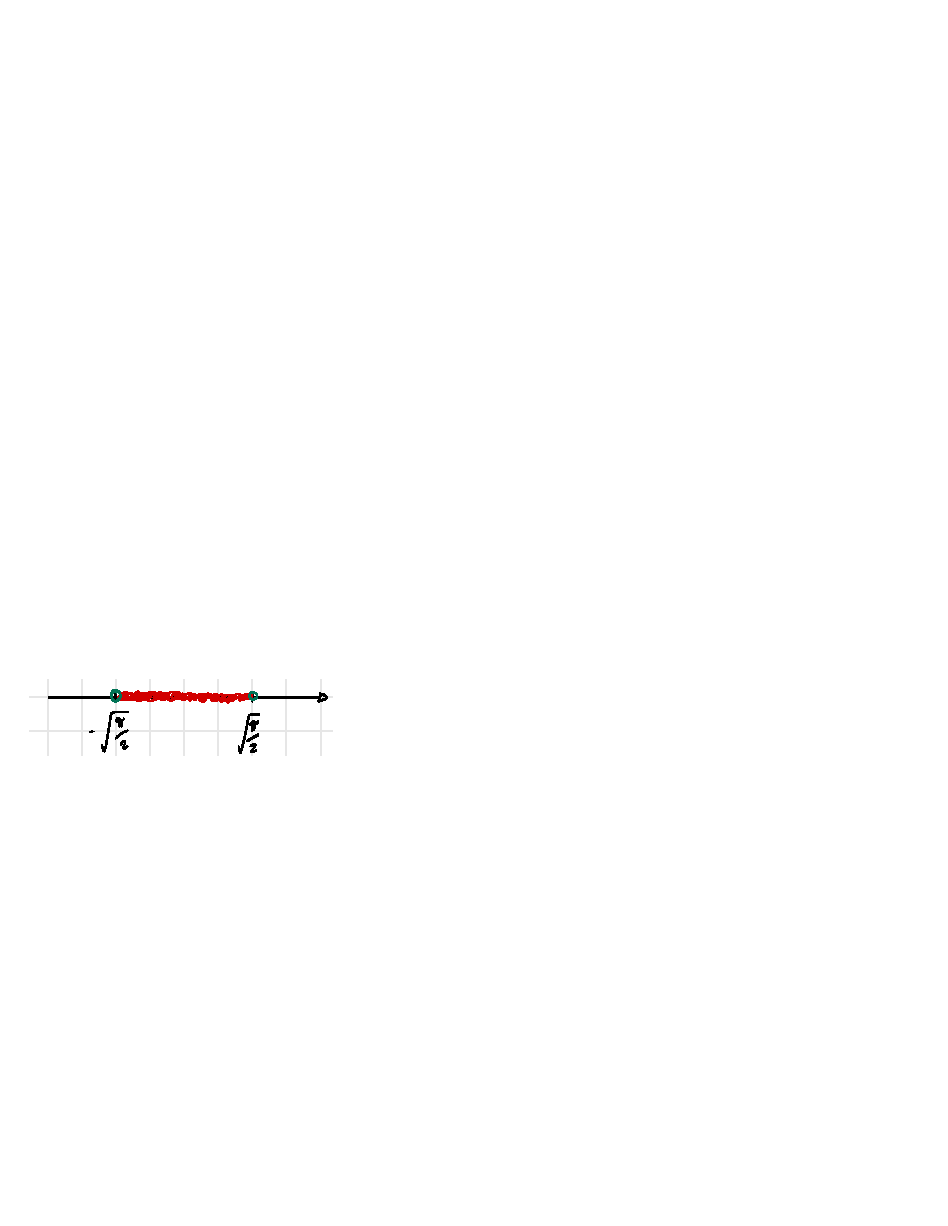
\includegraphics[width=0.7\textwidth]{img/intervallo_max_eg.pdf}
		\caption{Intervallo massimale delle soluzioni.}
	\end{figure}
\end{document}